\documentclass[12pt]{article}
\usepackage[utf8]{inputenc}
\usepackage[letterpaper, margin=1in]{geometry}
\usepackage{tabularx}
\usepackage{caption}
\usepackage{graphicx}
\usepackage{rotating}
\usepackage{tikz}
\usepackage{float}

\setlength{\parindent}{0em}
\renewcommand{\arraystretch}{1.25}
% Title Block
\title{
    CS4341: Bec-Man System Design \\
    \large The MetaStable Flip-Flops}
\author{Carson Page \and Husna Chaudhary}
\date{Fall 2019}
\begin{document}
\begin{titlepage}
    \maketitle
\end{titlepage}
\tableofcontents
\cleardoublepage
\listoftables
\listoffigures
\newpage

\setlength{\parskip}{0.5em}

\section{Parts List}
The parts list given here are derived from Vivado 2019.1, during the RTL
expansion phase of synthesis. If built from discrete logic, these listed
components would approximate the real world components necessary to build the
system. Following it is an implementation report for a Xilinx Artix-7 FPGA.

\newpage
\begin{center}
\captionof{table}{\textbf{RTL Parts List}}
\begin{tabular}{ ||c|l|| }
    \hline
    Part Name & Count \\
    \hline
        2 Input, 12 Bit Adder & 1 \\ 
        2 Input, 11 Bit Adder & 1 \\  
        2 Input, 10 Bit Adder & 8 \\  
        2 Input,  4 Bit Adder & 2 \\  
        2 Input,  2 Bit Adder & 1 \\
        \hline
        12 Bit Register & 1 \\
        11 Bit Register & 1 \\  
        10 Bit Register & 4 \\
        8 Bit Register & 3 \\
        6 Bit Register & 2 \\
        5 Bit Register & 2 \\
        4 Bit Register & 3 \\  
        3 Bit Register & 2 \\
        2 Bit Register & 4 \\
        1 Bit Register & 13 \\
        \hline
        1K Single Port RAM & 2 \\
        \hline
        2 Input,      50 Bit,        Mux & 2 \\
        \multicolumn{2}{||c||}{\textbf{NOTE:} This can be replaced with async ROM chip:} \\
        65 Input,     16 Bit,        Mux & 1     \\ 
         2 Input,     12 Bit,        Mux & 1     \\
         2 Input,     11 Bit,        Mux & 1     \\
         2 Input,     10 Bit,        Mux & 12    \\
         5 Input,     10 Bit,        Mux & 2     \\
         2 Input,      8 Bit,        Mux & 7     \\
         6 Input,      6 Bit,        Mux & 1     \\
         2 Input,      6 Bit,        Mux & 1     \\
         2 Input,      4 Bit,        Mux & 4     \\
         3 Input,      4 Bit,        Mux & 4     \\
         5 Input,      3 Bit,        Mux & 1     \\
         5 Input,      1 Bit,        Mux & 4     \\
         2 Input,      1 Bit,        Mux & 11    \\
         3 Input,      1 Bit,        Mux & 1  \\
    \hline
\end{tabular}
\end{center}

\newpage
\begin{center}
\captionof{table}{\textbf{Artix-7 Implementation}}
\begin{tabularx}{\linewidth}{ ||c|l|X|| }
    \hline
    Part Name & Count & Description\\
    BUFG     &     1  & Global clock buffer. Used to insert a signal onto the FPGA's
    global clock tree. \\
    CARRY4   &     5  & Carry logic between LUTs in different slices. Used to
    implement high-speed ripple-carry adders in fabric.\\
    LUT1     &     4  & 1-input, 1-output lookup table, generic logic function. \\
    LUT2     &    18  & 2-input, 1-output lookup table, generic logic function. \\
    LUT3     &    40  & 3-input, 1-output lookup table, generic logic function. \\
    LUT4     &    24  & 4-input, 1-output lookup table, generic logic function. \\
    LUT5     &    35  & 5-input, 1-output lookup table, generic logic function. \\
    LUT6     &   102  & 6-input, 1-output lookup table, generic logic function. \\
    MUXF7    &    14  & General-Purpose Multiplexer. \\
    MUXF8    &     3  & General-Purpose Multiplexer. \\
    RAM32X1S &   100  & Fabric distributed ROM. Used to store data on-masse near
    computation without Block RAM overhead. \\
    FDRE     &   121  & Synchronous Edge-Triggered D-Flip Flop with Reset
    Signal. \\
    FDSE     &    11  & Synchronous Edge-Triggered D-Flip Flop with Set Signal. \\
    IBUF     &     6  & Input Buffer. Used to bring signals into the FPGA. \\
    OBUF     &    26  & Output Buffer. Used to bring signals into the FPGA. \\
    \hline
\end{tabularx}
\end{center}

\section{Module Descriptions and Listing}
Each used module is documented here with a high-level description and its
function. Detailed port listings follow in the next section.

\subsection{Game State Engine (game\_state.sv)}
The game state is where the "game" proper lives in logic. It is a combination of
a sequencing state machine, along with a decision path, that produces the
outputs required for the video layer.

The logic is keyed into different states annotated by a $state$ enum. This state
advanced unconditionally except when initially leaving the "idle" state. The
condition for leaving the idle state is a positve edge on the state engine
enable. This causes the game to update once per frame, allowing for consistant
timing on based on the screen refresh rate.

\subsection{Video Timing Generator (vtg.sv)}
The Video Timing Generator is a critical component of timing and sequencing both the game state and
video engine. Its principal role is for creating the necessary signals to output
to a VGA display for video output. It also outputs screen coordinates internally
to the rest of the design to allow the video systems to have an easy reference 
to the currently drawn pixels.

The VTG is also used for sequencing the handover between the game state and the
video subsystem. The vertical blanking signal is routed to the enable of the
game state, and its inverse to the sprite engines. This allows game state to
remain constant while the screen is drawing preventing visual artifacts, and
provides for timing based on the screen refresh rate. The horizontal blanking
signal is also used to properly sequence the sprite engines in addition to the
vblank signal.

\subsection{Sprite Generators (becman\_sprite.sv and map\_sprite.sv)}
The sprite generators form the core of the video engine. They are a purely
feedforward system, taking information from the VTG and the game state to blit
pixels to the screen. Both the Bec-Man and Map sprite engine use a series of
ROMs or RAMs to hold the graphics data.

When a sprite engine decides to output a pixel, it emits a valid signal and the
color information. This is fed into the video arbiter as a final processing
step.

\subsection{Map RAM (map\_ram.sv)}
This hold the current map state. In our current implementation, the write signal
is always held low treating it like a ROM, but it supports writes to enable a
dynamic update of the map for future implementation of bonuses or dots.

This was broken out as a seperate module to be easily reused in both the game
state engine and the map sprite subsystems.

\subsection{Video Arbiter (video\_arbiter.sv)}
The video arbiter is the last component before sending the signal to the
display. It decides for each pixel which sprite takes priority and has its color
drawn to screen. This is done with a fixed priority based on input port.

This is required as the video subsystem contains no framebuffer in memory,
requiring it to generate video in realtime without a compositing step. This
requires we select the appropriate signal in realtime as well. Since the valid
signals are able to be toggled on a pixel by pixel basis, this allows a crude
form of transparancy by allowing a lower priority pixel to come through at that
time if a higher priortity pixel is not being shown. If no sprite engine is
attempting to write data at that time, the arbiter outputs black to set a global
background color.

\subsection{TMDS Encoder (tmds\_encoder.sv)}
\textbf{NOTE:} This module is unused in the design as implemented, but noted here for reference. It does
not appear later in the document as such.

The TMDS encoders function is to translate VGA signals into one that can be
output using an FPGA's DDR I/O ports to a HDMI display. This allows the internal
design to work with simple signals, and only apply the relatively complex TMDS
encoding at a final processing stage.

Since the design was not sucessfully put onto an FPGA by project completion, this module was not used in the final
test bench.

\subsection{Primary Testbench (tb/drawing\_test.sv)}
This is the primary testbench file that provides for the top level design. This
is fed into Verilator to make a working cycle-accurate of the verilog as if it
was on a hardware device like an FPGA or ASIC. It additionally breaks out the
signals to enable the VGASim component of the Verilator to read the display information.

\section{System Listing}

Each of the modules Inputs, Outputs, and Notable Registers are listed here. This
also satisfies the interface listing requirements as each module describes how
it may interconnect with other modules.

\subsection{Defined Types}

We defined multiple new types to assist in development. These are replicated
commonly in the next sections.

\begingroup
\captionof{table}{\textbf{Defined Types}}
\begin{tabularx}{\linewidth}{ ||c|c|X|| }
    \hline
    Type Name   & Width     & Description \\
    \hline
    s\_width\_t & clogb2(SCREEN\_WIDTH) & Generated type that fits the visible
    screen width. \\
    s\_height\_t & clogb2(SCREEN\_HEIGHT)  & Generated type that fits the visible
    screen height. \\
    coord\_t     &  s\_width\_t + s\_height\_t & XY Coordinate Pair. \\
    rgb\_t      & [23:0]    & Packed struct representing 8:8:8 RGB color. \\
    \hline
\end{tabularx}
\endgroup

\newpage
\subsection{Input Listing}
Each module has its input(s) name, type, and description listed in a table
below. Inputs that are prevelent and share the same semantic meaning are in Table
\ref{tab:input_common}.

\begingroup
\captionof{table}{\textbf{Common Inputs}}
\label{tab:input_common}
\begin{tabularx}{\linewidth}{ ||c|c|X|| }
    \hline
    Name & Type & Description \\
    \hline
    i\_clk & logic & Global system clock tree. All logic is driven off of this
    or a derived clock from a PLL / MMCM module. \\
    i\_rst & logic & Active high reset. Module must reset registers and/or
    outputs to known base state on activation. \\
    i\_en   & logic & Active high clock enable. Registers part of the data path
    should only update when activated. Control registers or edge detect
    registers \emph{may} not be disabled on a low if necessary for proper function. \\
    \hline
\end{tabularx}
\endgroup

\vspace{0.5in}
\begingroup
\captionof{table}{\textbf{Video Timing Generator Inputs (vtg)}}
\label{tab:input_vtg}
\begin{tabularx}{\linewidth}{ ||c|c|X|| }
    \hline
    Name & Type & Description \\
    \hline
    ACTIVE\_WIDTH & parameter & The width of the visible area of the display. \\
    ACTIVE\_HEIGHT & parameter & The height of the visible area of the display.
    \\
    V\_FRONT\_PORCH & parameter & Vertical front porch of the timing spec in
    lines. \\
    V\_BACK\_PORCH & parameter & Vertical back porch of the timing spec in
    lines. \\
    V\_PULSE & parameter & Length of vertical sync pulse in lines. \\
    V\_POL & parameter & Defines if the module outputs a active high/low
    vertical sync pulse. \\
    H\_FRONT\_PORCH & parameter & Horizontal front porch of the timing spec in
    pixels. \\
    H\_BACK\_PORCH & parameter & Horizontal back porch of the timing spec in
    pixels. \\
    H\_PULSE & parameter & Length of horizontal sync pulse in pixels. \\
    H\_POL & parameter & Defines if the module outputs a active high/low
    horizontal sync pulse. \\
    \hline
\end{tabularx}
\endgroup

\vspace{0.5in}
\begingroup
\captionof{table}{\textbf{Game State Engine Inputs (game\_state)}}
\label{tab:input_game_state}
\begin{tabularx}{\linewidth}{ ||c|c|X|| }
    \hline
    Name & Type & Description \\
    \hline
    i\_joystick & logic [3:0] & Joystick Input, lowest bit represents the left
    direction. Successive bits represent the next cardinal direction in a
    counter-clockwise manner. The zero vector represents no input. \\
    \hline
\end{tabularx}
\endgroup

\vspace{0.5in}
\begingroup
\captionof{table}{\textbf{Bec-Man Sprite Generator Inputs (becman\_sprite)}}
\label{tab:input_becman_state}
\begin{tabularx}{\linewidth}{ ||c|c|X|| }
    \hline
    Name & Type & Description \\
    \hline
    i\_rotate & logic [2:0] & Dictates the rotation of the becman sprite. This
    value must be held constant while the enable is active. \\
    i\_becman & coord\_t & The screen top-left referenced screen coordnates of the
    becman sprite. This value must be held constant while the enable is active. \\
    i\_screen & coord\_t & The pixel currently being blited to the screen. This is
    used to determine if the sprite contains an active pixel at the translated
    coordinates. \\
    \hline
\end{tabularx}
\endgroup

\vspace{0.5in}
\begingroup
\captionof{table}{\textbf{Map Sprite Generator Inputs (map\_sprite)}}
\label{tab:input_map_sprite}
\begin{tabularx}{\linewidth}{ ||c|c|X|| }
    \hline
    Name & Type & Description \\
    \hline
    i\_screen & coord\_t & The pixel currently being blited to the screen. This is
    used to determine if the sprite contains an active map element. \\
    \hline
\end{tabularx}
\endgroup

\vspace{0.5in}
\begingroup
\captionof{table}{\textbf{Map RAM Inputs (map\_ram)}}
\label{tab:input_map_ram}
\begin{tabularx}{\linewidth}{ ||c|c|X|| }
    \hline
    Name & Type & Description \\
    \hline
    i\_write & logic & Sets if the RAM is in read/write mode. \\
    i\_tile\_x & logic [5:0] & The X address of the map tile. \\
    i\_tile\_y & logic [4:0] & The Y address of the map tile. \\
    \hline
\end{tabularx}
\endgroup

\vspace{0.5in}
\begingroup
\captionof{table}{\textbf{Video Arbiter Inputs (video\_arbiter)}}
\label{tab:input_video_arbiter}
\begin{tabularx}{\linewidth}{ ||c|c|X|| }
    \hline
    Name & Type & Description \\
    \hline
    i\_vsync & logic & Passthrough input for vsync to keep it in sync with the
    muxed video signal. \\
    i\_hsync & logic & Passthrough input for hsync to keep it in sync with the
    muxed video signal. \\
    i\_req & logic [1:0] & Arbiter request input, MSB takes priority. A zero
    vector indicates to draw the default color. \\
    i\_vport & rgb\_t [1:0] & Array of input video ports. These are muxed
    depedent on the decided input from the arbiter. \\
    \hline
\end{tabularx}
\endgroup

%
% OUTPUT LIST
%
\subsection{Output Listing}
Each module has its output(s) name, type, and description listed in a table
below.

\begingroup
\captionof{table}{\textbf{Video Timing Generator Outputs (vtg)}}
\label{tab:output_vtg}
\begin{tabularx}{\linewidth}{ ||c|c|X|| }
    \hline
    Name & Type & Description \\
    \hline
    o\_hsync & logic & Horizontal sync pulse output. \\
    o\_vsync & logic & Vertical sync pulse output. \\
    o\_hblank & logic & Active high when the display is in the horizontal blanking
    period. \\
    o\_vblank & logic & Active high when the display is in the vertical blanking
    period. \\
    o\_blank & logic & $o\_hblank \mid \mid o\_vblank$ \\
    o\_screen & coord\_t & The current XY pixel being sent to the display, in
    relation to the sync pulses. \\
    \hline
\end{tabularx}
\endgroup

\vspace{0.5in}
\begingroup
\captionof{table}{\textbf{Game State Engine Outputs (game\_state)}}
\label{tab:output_game_state}
\begin{tabularx}{\linewidth}{ ||c|c|X|| }
    \hline
    Name & Type & Description \\
    \hline
    o\_becman & coord\_t & Where the Bec-Man sprite should be drawn on the
    display, as derived from the internal state. \\
    o\_becman\_dir & logic [2:0] & The direction of the Bec-Man sprite should be
    rotated to, as derived from the internal state. \\
    \hline
\end{tabularx}
\endgroup

\vspace{0.5in}
\begingroup
\captionof{table}{\textbf{Bec-Man Sprite Generator Outputs (becman\_sprite)}}
\label{tab:output_becman_sprite}
\begin{tabularx}{\linewidth}{ ||c|c|X|| }
    \hline
    Name & Type & Description \\
    \hline
    o\_valid & logic & Active high when the video system should blit pixels from
    this sprite. \\
    o\_color & rgb\_t & The color to display when $o\_valid$ is high. \\
    \hline
\end{tabularx}
\endgroup

\vspace{0.5in}
\begingroup
\captionof{table}{\textbf{Map Sprite Generator Outputs (map\_sprite)}}
\label{tab:output_map_sprite}
\begin{tabularx}{\linewidth}{ ||c|c|X|| }
    \hline
    Name & Type & Description \\
    \hline
    o\_valid & logic & Active high when the video system should blit pixels from
    this sprite. \\
    o\_color & rgb\_t & The color to display when $o\_valid$ is high. \\    
    \hline
\end{tabularx}
\endgroup

\newpage
\begingroup
\captionof{table}{\textbf{Map RAM Outputs (map\_ram)}}
\label{tab:output_map_ram}
\begin{tabularx}{\linewidth}{ ||c|c|X|| }
    \hline
    Name & Type & Description \\
    \hline
    o\_tile\_value & logic & Active high when a tile is present at the input
    coordinates. \\
    \hline
\end{tabularx}
\endgroup

\vspace{0.5in}
\begingroup
\captionof{table}{\textbf{Video Arbiter Outputs (video\_arbiter)}}
\label{tab:output_video_arbiter}
\begin{tabularx}{\linewidth}{ ||c|c|X|| }
    \hline
    Name & Type & Description \\
    \hline
    o\_vport & rgb\_t & The selected video signal based on the input request and
    priority level. \\
    o\_hsync & logic & Passthrough of the input hsync signal for timing
    purposes. \\
    o\_vsync & logic & Passthrough of the input vsync signal for timing purposes. \\
    \hline
\end{tabularx}
\endgroup

%
% Register List
%
\subsection{Register Listing}
Each module has its registers wires(s) name, type, and description listed in a table
below, where applicable.

\begingroup
\captionof{table}{\textbf{Video Timing Generator Interfacing (vtg)}}
\label{tab:interface_vtg}
\begin{tabularx}{\linewidth}{ ||c|c|X|| }
    \hline
    Name & Type & Description \\
    \hline
    r\_pix\_cnt & logic [clogb2(H\_TOTAL-1):0] & Master horizontal count state.
    \\
    r\_line\_cnt & logic [clogb2(V\_TOTAL-1):0] & Master vertical count state.
    \\
    \hline
\end{tabularx}
\endgroup

\vspace{0.5in}
\begingroup
\captionof{table}{\textbf{Game State Engine Interfacing (game\_state)}}
\label{tab:interface_game_state}
\begin{tabularx}{\linewidth}{ ||c|c|X|| }
    \hline
    Name & Type & Description \\
    \hline
    r\_en\_edge & logic [1:0] & Register used to detect the enable edge on
    $vblank$ to advance states. \\
    r\_joystick & logic [1:0] & Latches input during state computation. \\
    will\_collide & logic & Stores weather becman will collide this frame. \\
    r\_next\_pos & coord\_t & Stores becman's position to be drawn next frame
    during computation. \\
    r\_next\_dir & logic [2:0] & Stores the computed rotation for the becman
    sprite during computation. \\
    state & state\_t & Keeps track of the current state of the micro-sequencer FSM.\\
    \hline
\end{tabularx}
\endgroup

\newpage

\vspace{0.5in}
\begingroup
\captionof{table}{\textbf{Bec-Man Sprite Generator Interfacing (becman\_sprite)}}
\label{tab:output_becman_sprite}
\begin{tabularx}{\linewidth}{ ||c|c|X|| }
    \hline
    Name & Type & Description \\
    \hline
    r\_pix\_count & logic [3:0] & Sprite horizontal count state.
    \\
    r\_line\_count & logic [3:0] & Sprite vertical count state. \\
    x/yvalid & logic & Determines weather sprite should enable output.
    \\
    \hline
\end{tabularx}
\endgroup

%
% MODE LIST
%
\subsection{Mode Listing}
The system contains several modal systems listed here.

\subsubsection*{Top Level}
The primary system has two modes, state update and rendering. These are
controlled by the vtg $o\_vblank$, $o\_hblank$, and $o\_blank$ signals in a variety
of ways. In general, it works as follows:

\begingroup
\captionof{table}{\textbf{Top Level Drawing Modes}}
\label{tab:top_level_video_mode}
\begin{tabularx}{\linewidth}{ ||c|X|| }
    \hline
    $vblank$ & Description \\
    \hline
    Logic High & System is in state update mode. The game state engine advances through a
    single cycle of the microsequencer. Conversely, video output is disabled as
    we are in the blanking period. \\
    Logic Low & System is in drawing mode. The state engine is halted, and the
    enables come alive for the sprite engines. These are further gated by the
    $o\_hblank$ signals to maintain horizontal drawing accuracy. \\
    \hline
\end{tabularx}
\endgroup

\subsubsection*{Map RAM}
The Map RAM can in theory be in two modes, read or write as controlled by
$i\_write$. However, this is currently hard-wired to read in the current implementation.

\newpage
\section{Circuit Diagrams}
The various circuit and state diagrams are included here on seperate pages. \\
\textbf{NOTE:} Vivado breaks up packed structs when generating diagrams, so a
wire of type $rgb\_t$ will be broken into three wires for the diagram, labled
each with an R, G, and B component. In addition, Vivado will postfix registers
with "\_reg".

\begin{sidewaysfigure}[htp]
    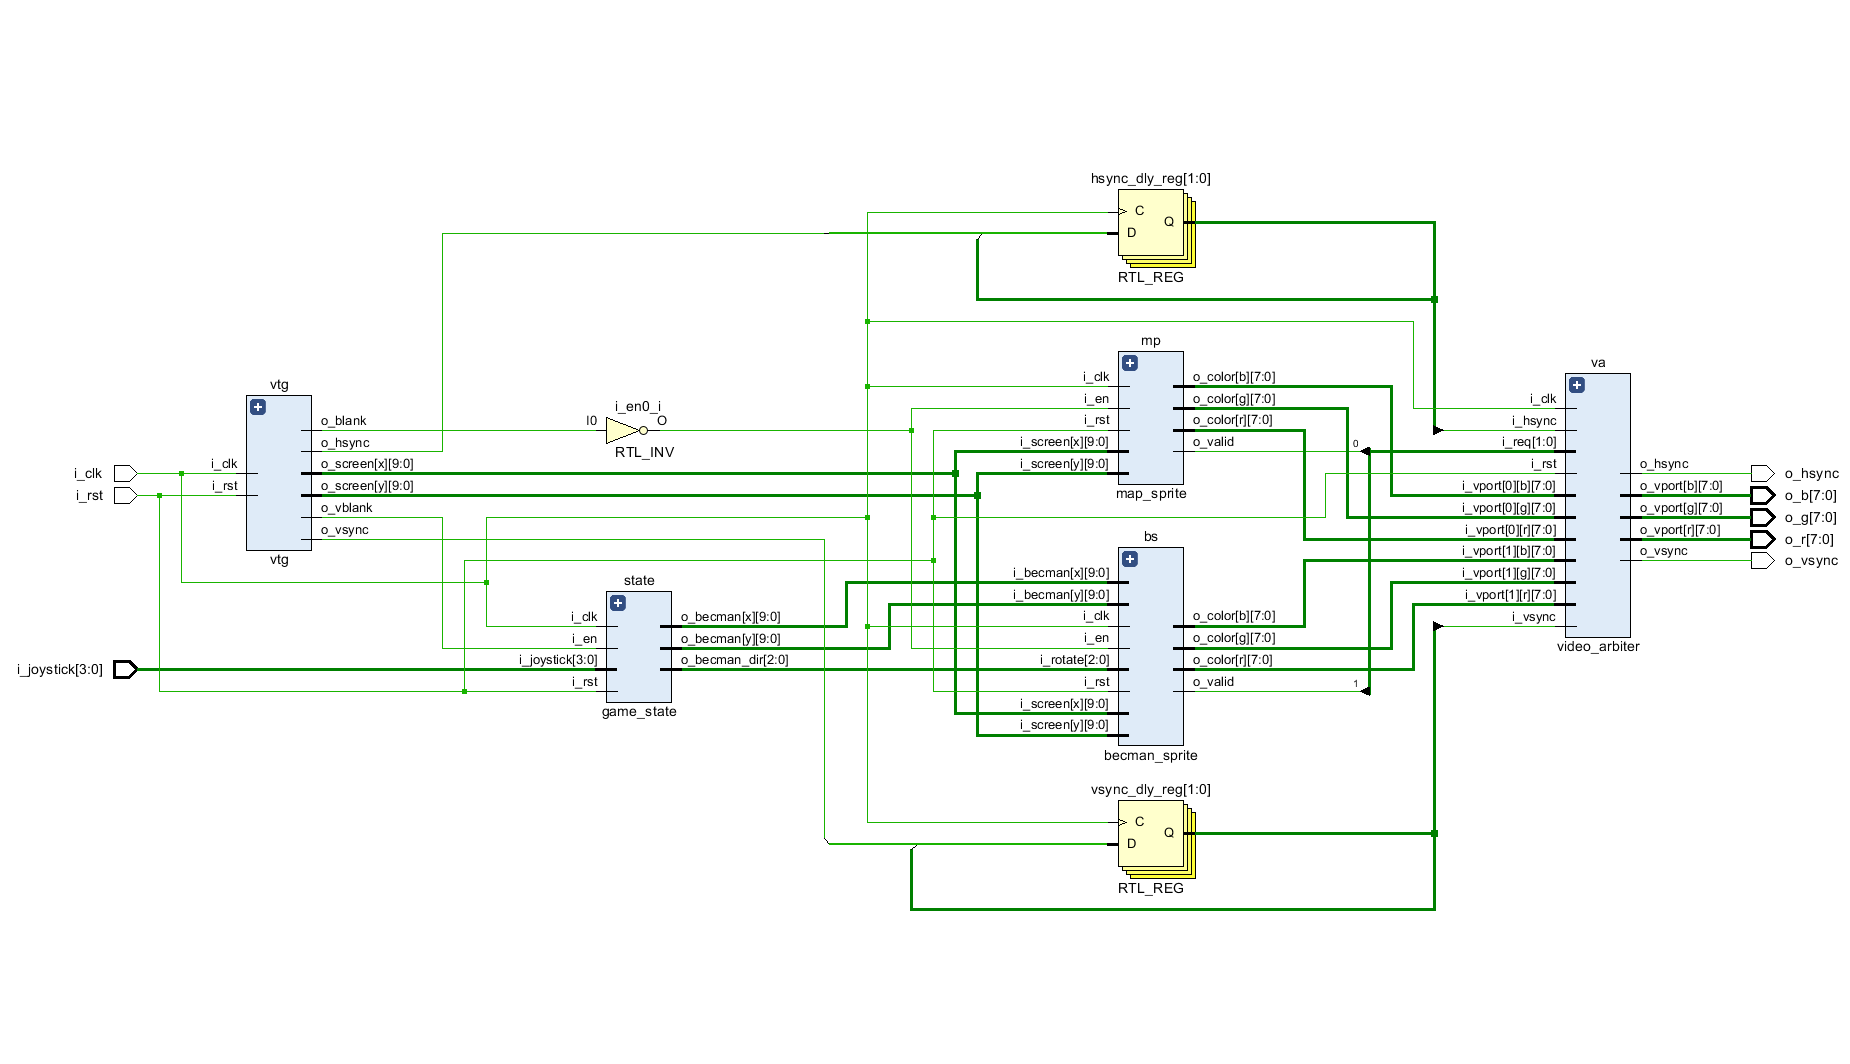
\includegraphics[width=\textwidth]{TopLevelDiagram.png}
    \caption{Top Level Block Diagram of the Bec-Man System.}
    \label{fig:LandscapeFigure}
\end{sidewaysfigure}

\begin{sidewaysfigure}[htp]
    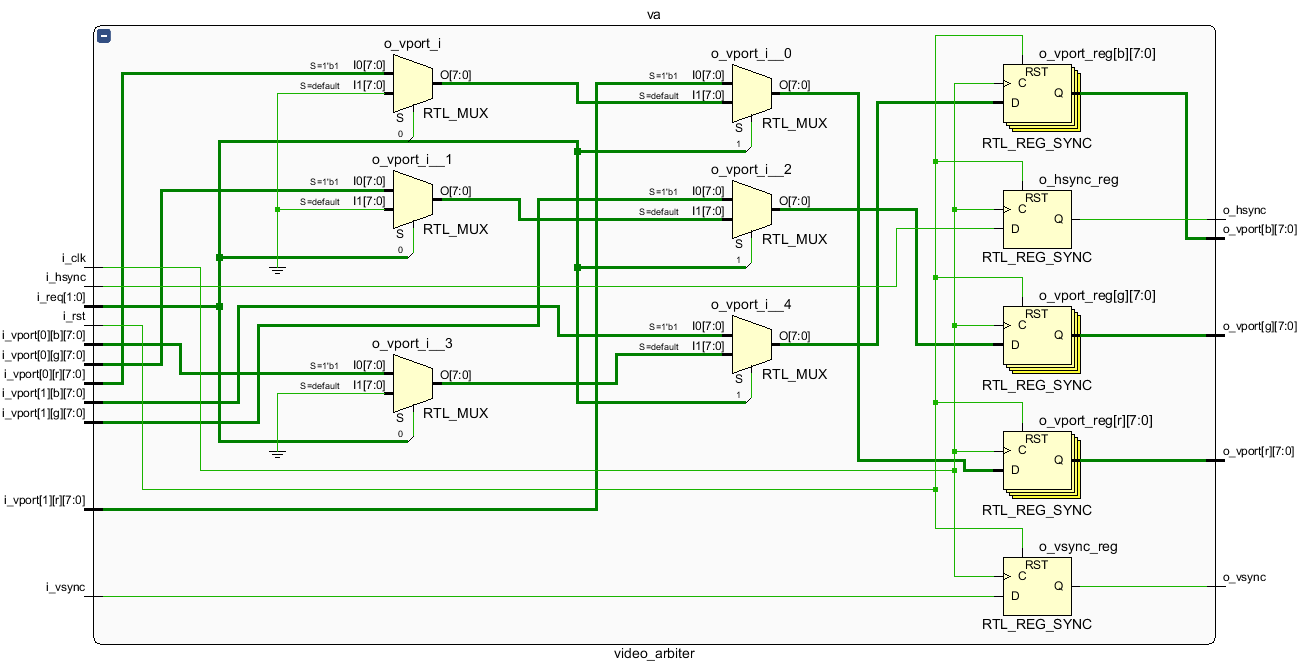
\includegraphics[width=\textwidth]{VideoArbiter.png}
    \caption{Video Arbiter}
    \label{fig:LandscapeFigure}
\end{sidewaysfigure}

\begin{sidewaysfigure}[htp]
    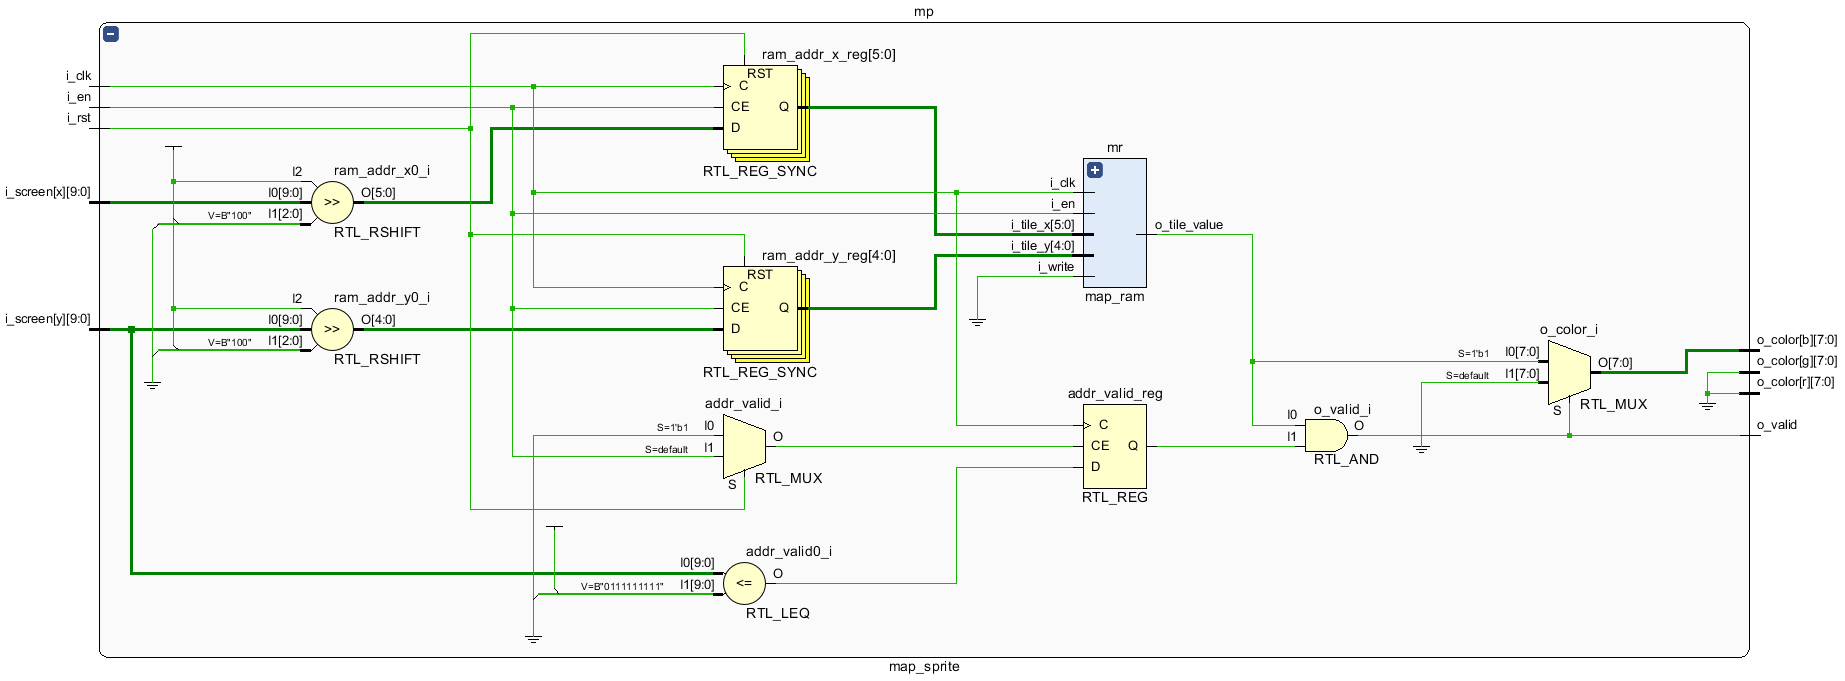
\includegraphics[width=\textwidth]{MapSprite.png}
    \caption{Map Sprite Engine}
    \label{fig:LandscapeFigure}
\end{sidewaysfigure}

\begin{sidewaysfigure}[htp]
    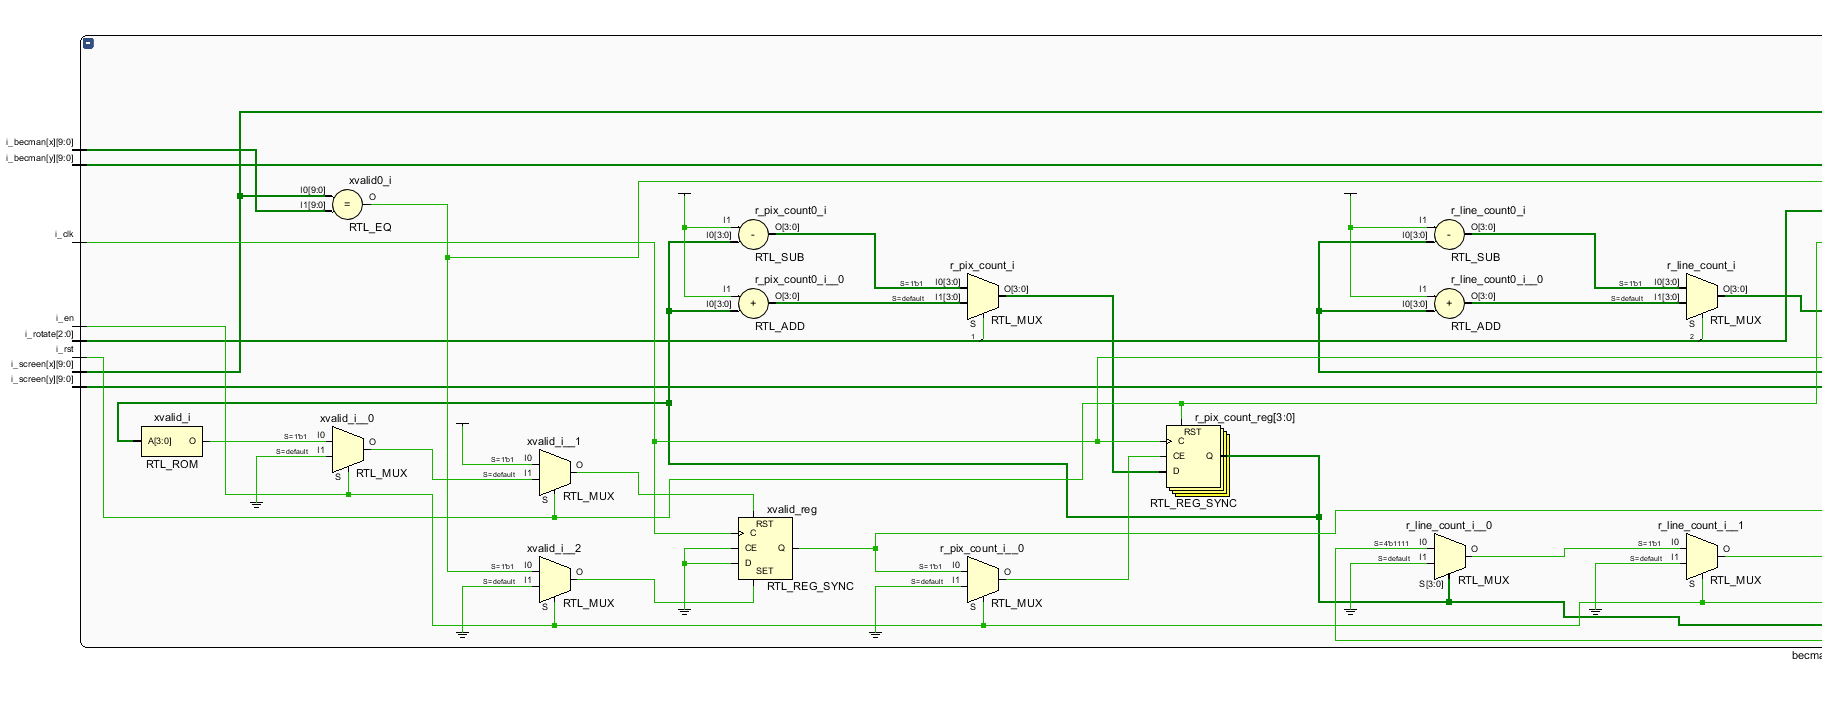
\includegraphics[width=\textwidth]{BecmanSpritePt1.png}
    \caption{Becman Sprite Engine}
    \label{fig:LandscapeFigure}
\end{sidewaysfigure}

\begin{sidewaysfigure}[htp]
    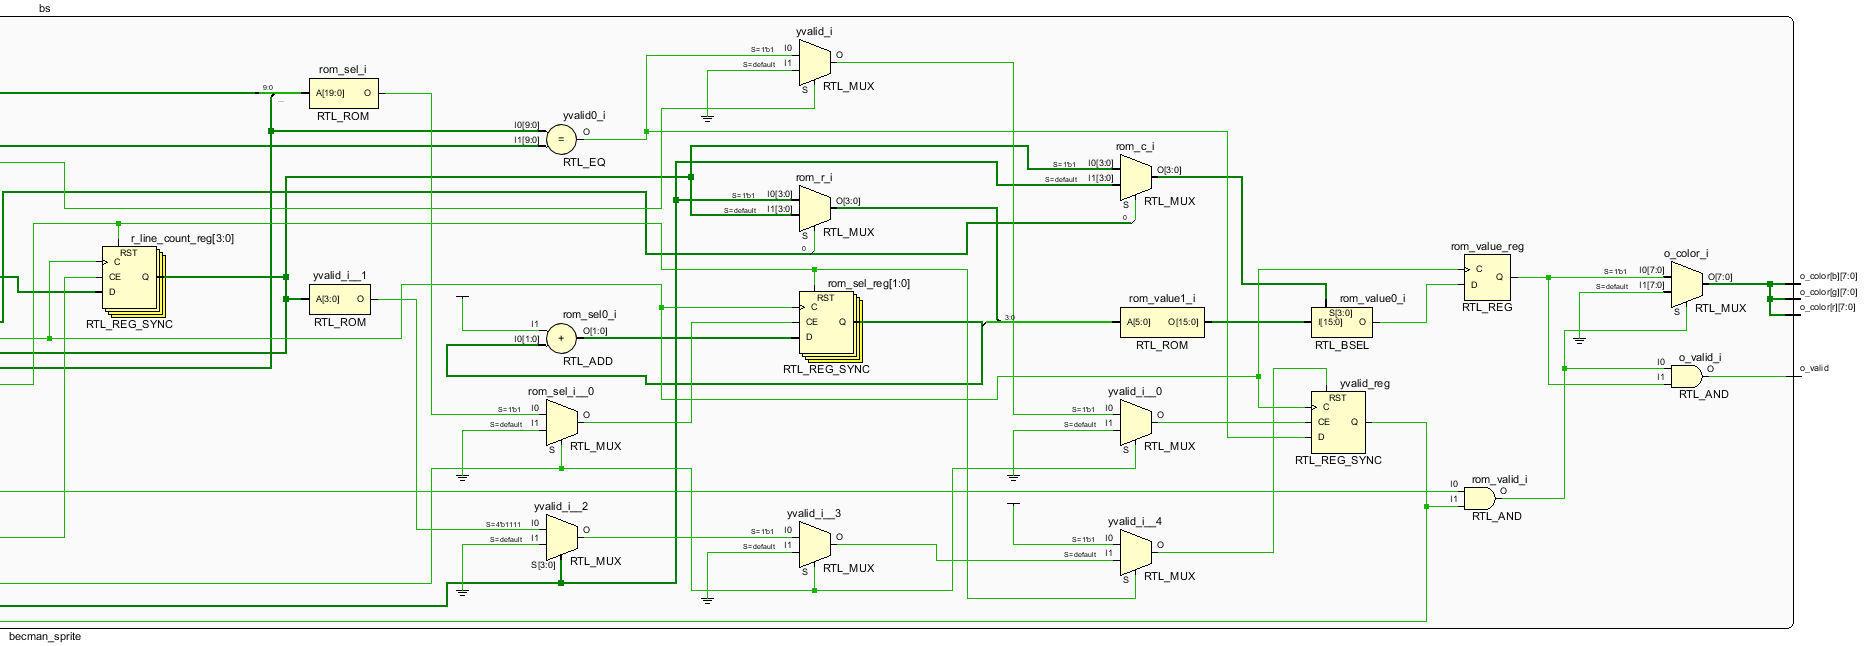
\includegraphics[width=\textwidth]{BecmanSpritePt2.png}
    \caption{Becman Sprite Engine Cont.}
    \label{fig:LandscapeFigure}
\end{sidewaysfigure}

\begin{sidewaysfigure}[htp]
    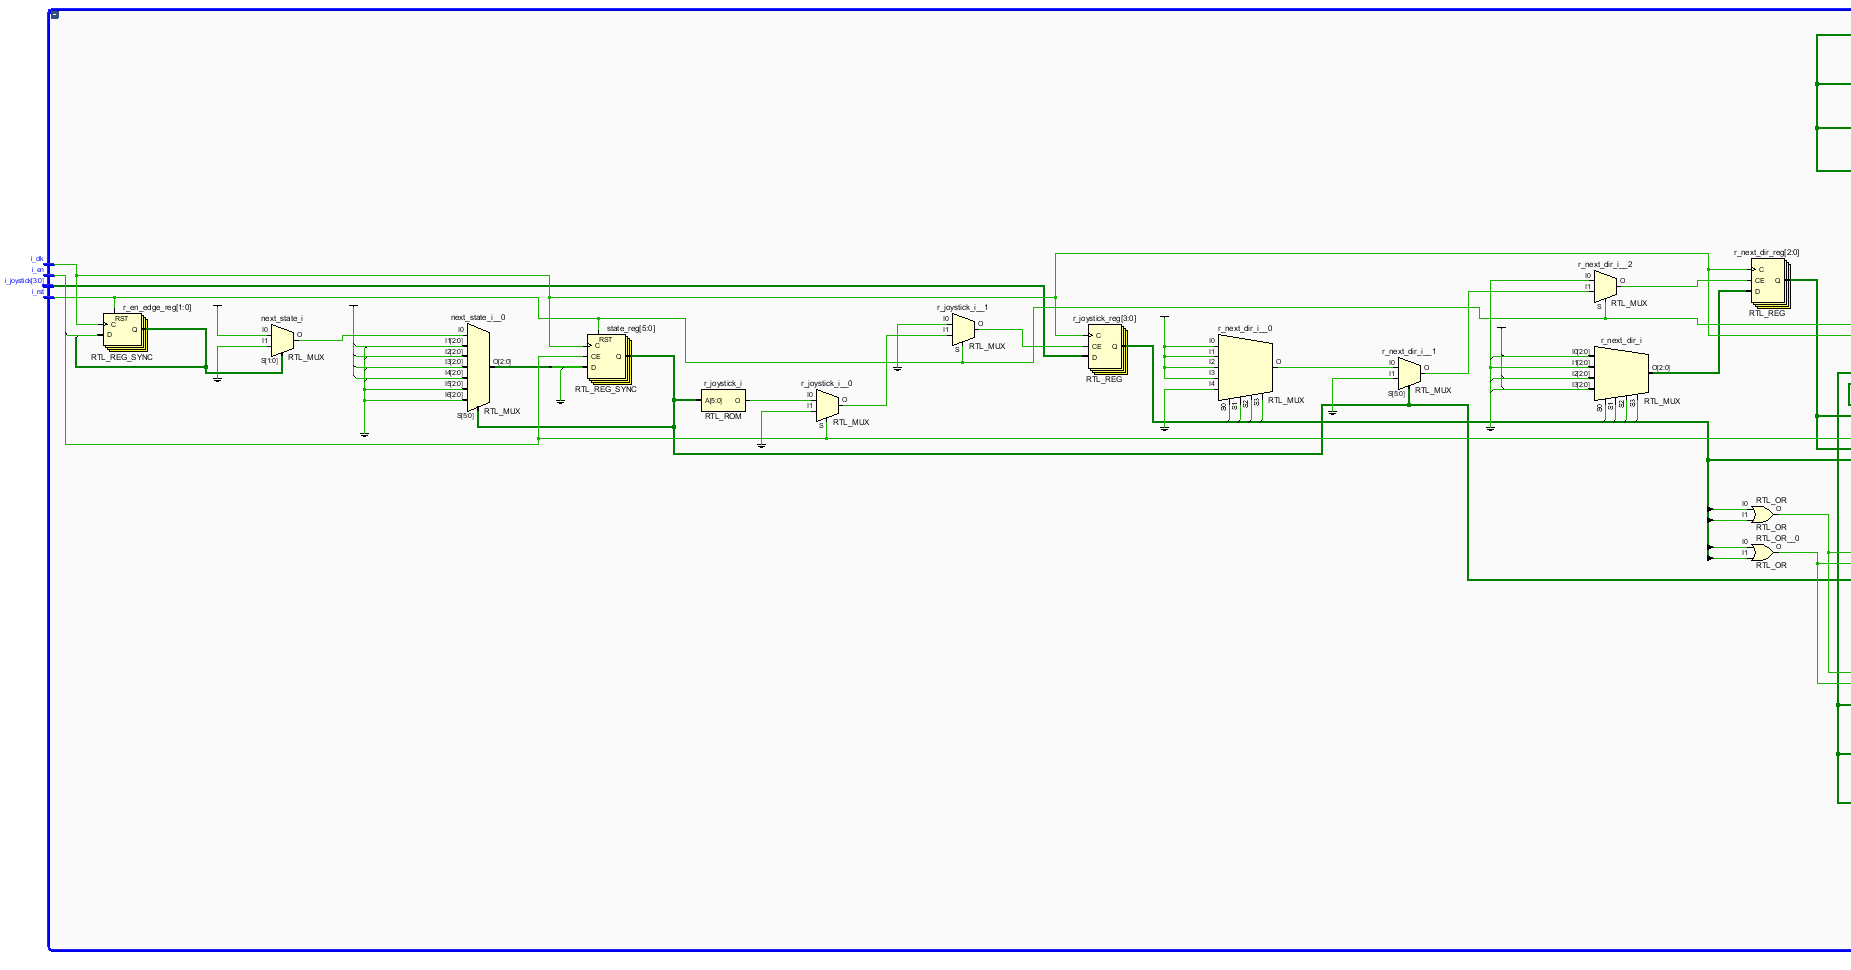
\includegraphics[width=\textwidth]{GameStatePt1.png}
    \caption{Game State Engine}
    \label{fig:LandscapeFigure}
\end{sidewaysfigure}

\begin{sidewaysfigure}[htp]
    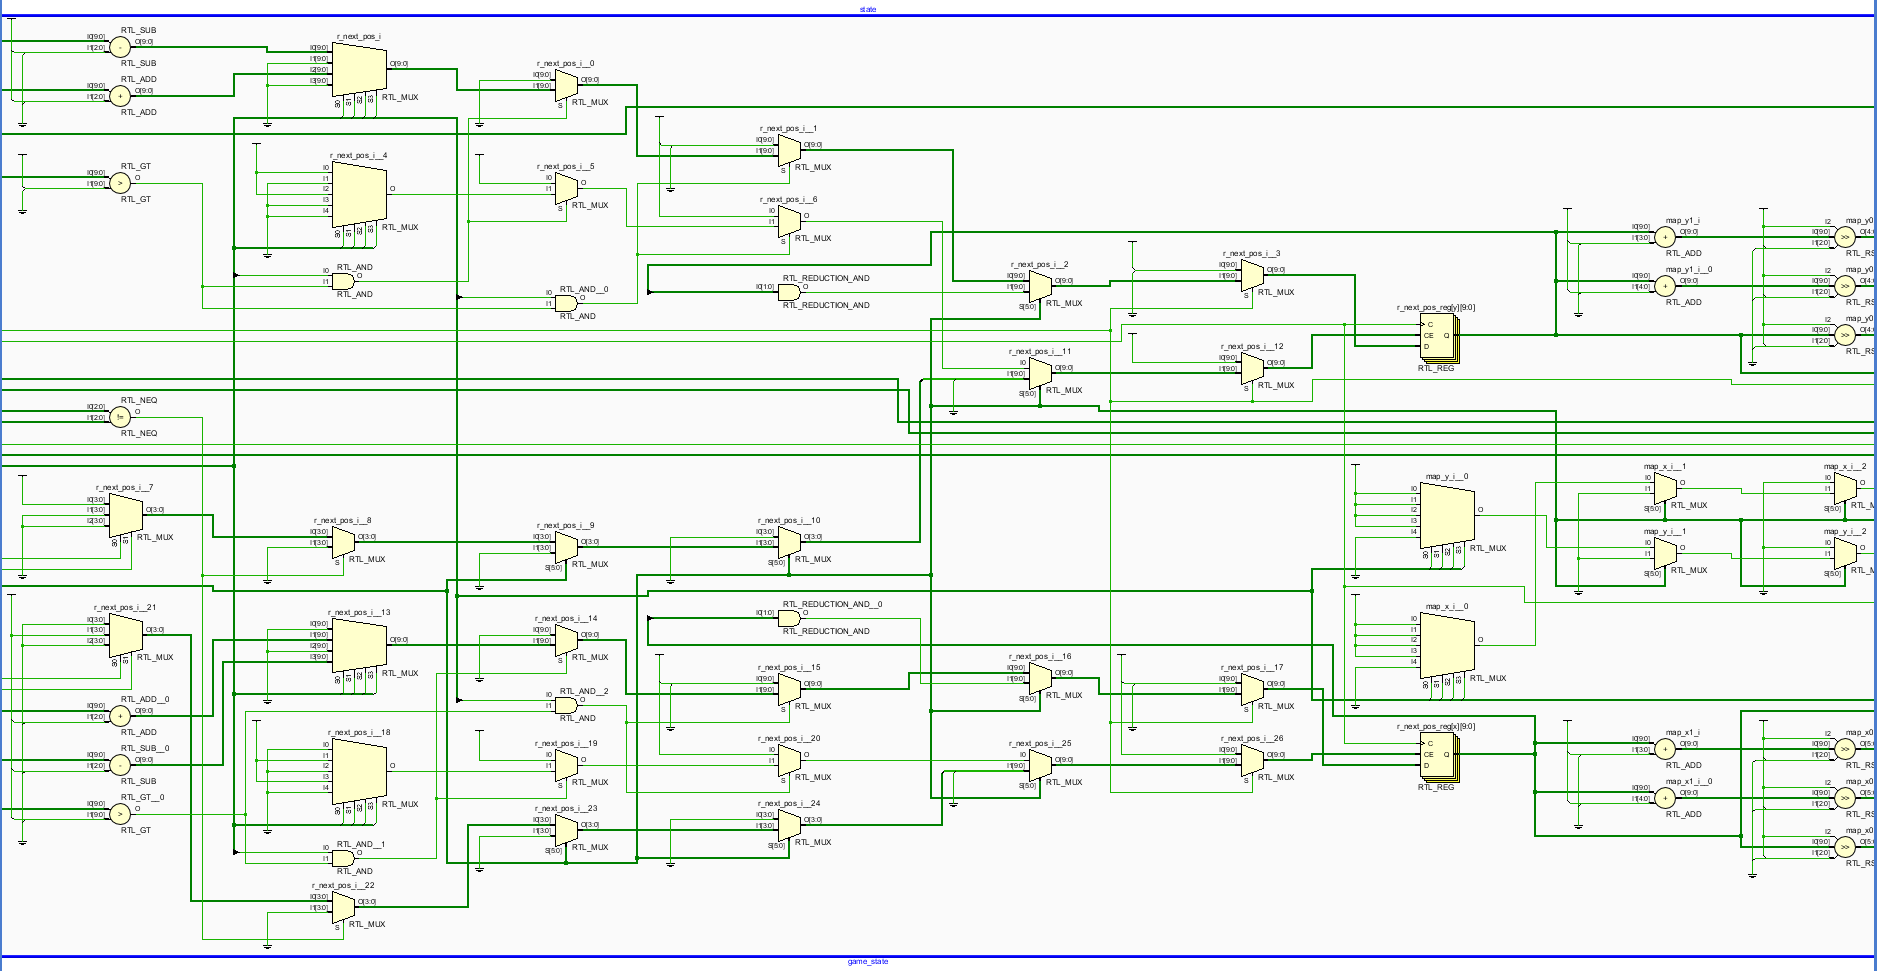
\includegraphics[width=\textwidth]{GameStatePt2.png}
    \caption{Game State Engine Cont.}
    \label{fig:LandscapeFigure}
\end{sidewaysfigure}

\begin{sidewaysfigure}[htp]
    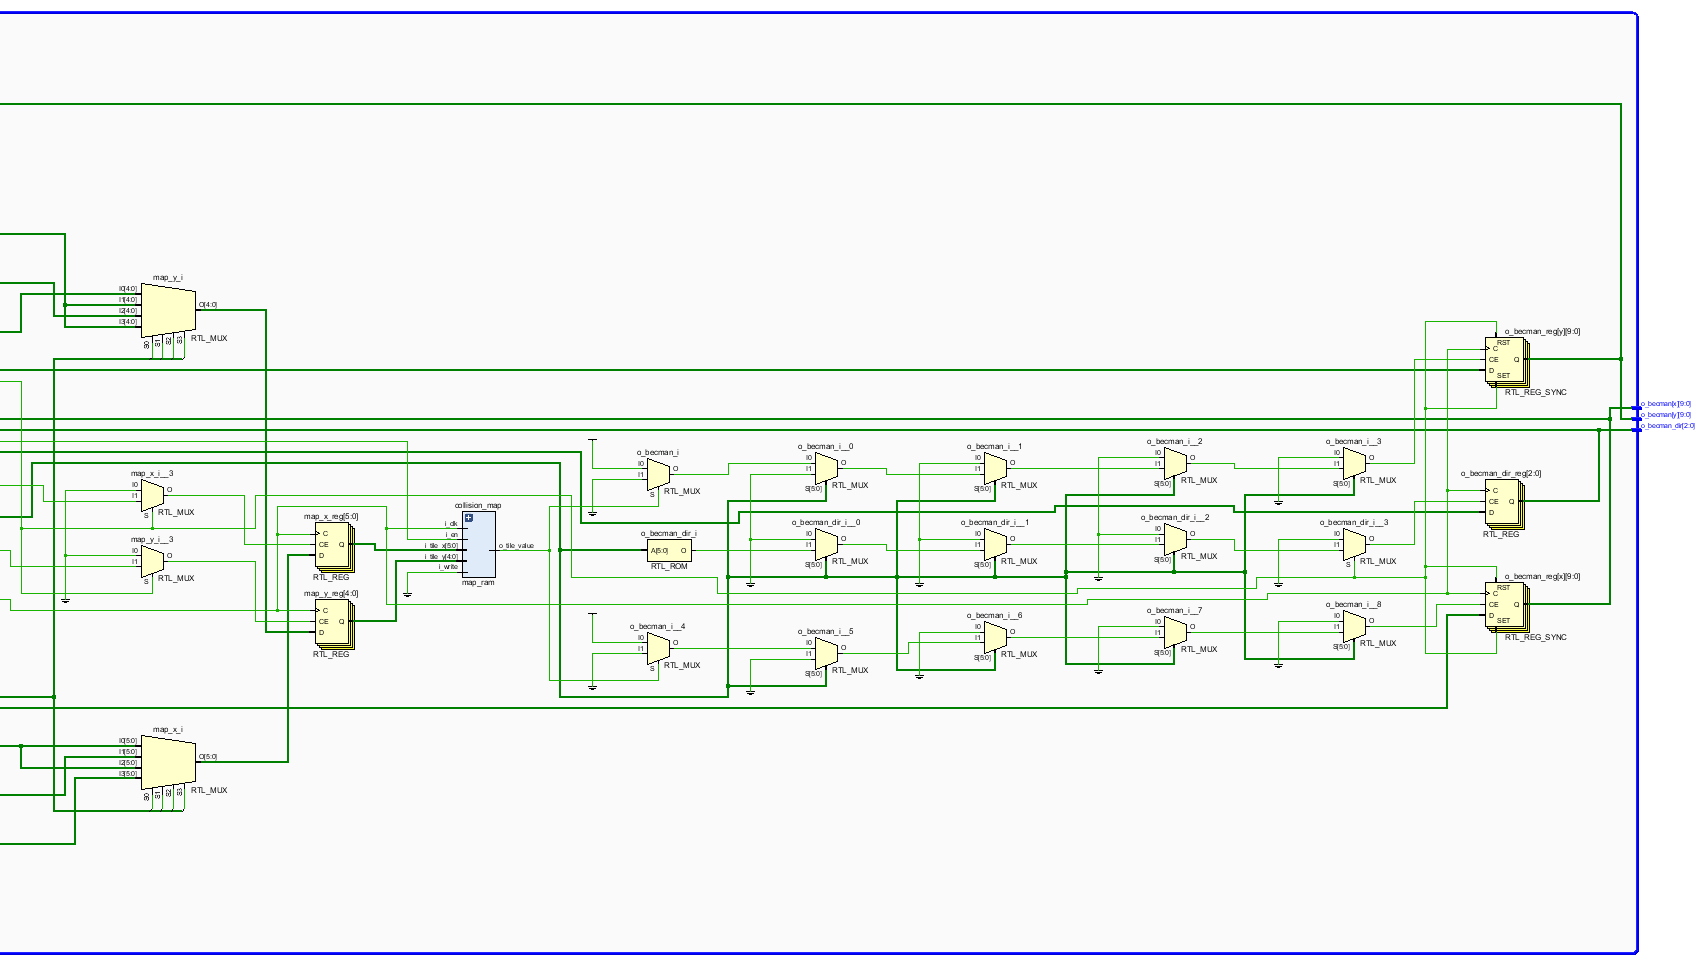
\includegraphics[width=\textwidth]{GameStatePt3.png}
    \caption{Game State Engine Cont.}
    \label{fig:LandscapeFigure}
\end{sidewaysfigure}

\begin{sidewaysfigure}[htp]
    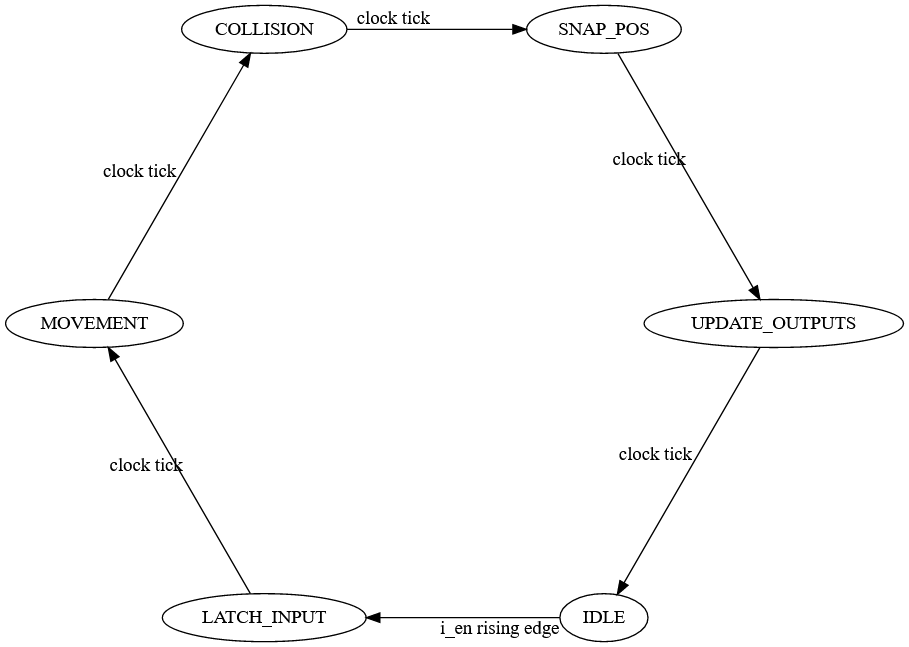
\includegraphics[width=\textwidth]{Sequencer.png}
    \caption{Sequencer State Machine}
    \label{fig:LandscapeFigure}
\end{sidewaysfigure}
\end{document}